\documentclass[conference]{IEEEtran}

\usepackage{cite}
\usepackage{amsmath,amssymb}
\usepackage{graphicx}
\usepackage{booktabs}
\usepackage{tabularx}
\usepackage{xcolor}
\usepackage{url}
\usepackage[hidelinks]{hyperref}

\urlstyle{same}

\newcommand{\placeholderbox}[2]{%
  \fbox{%
    \begin{minipage}[c][#1][c]{0.96\linewidth}
      \centering
      \vspace{0.4em}
      #2
      \vspace{0.4em}
    \end{minipage}
  }%
}

\newcommand{\includeorplaceholder}[3]{%
  \IfFileExists{#1}{%
    \includegraphics[width=\linewidth]{#1}%
  }{%
    \placeholderbox{#2}{#3}%
  }%
}

\newcommand{\resultplaceholder}[1]{\textcolor{red}{\textbf{[[#1]]}}}
\newcommand{\codefont}[1]{\texttt{#1}}

\title{Multimodal Vision-Language-Action Decision Support\\for False-Positive Safety Stops in Autonomous Guided Vehicles}

\author{
\IEEEauthorblockN{Vikas Rathore, Neha Anil Khot}
\IEEEauthorblockA{
Information Technology\\
Frankfurt University of Applied Sciences\\
Autonomous Intelligent Systems\\
vikas.rathore@stud.fra-uas.de\\
neha.khot@stud.fra-uas.de
}
}

\begin{document}

\maketitle

\begin{abstract}
False-positive safety stops are a routine source of friction in warehouse AGV operations. Proximity sensors appropriately err on the side of caution, but they cannot tell a dangerous obstacle from lightweight material such as wrapping film, paper debris, or hanging plastic. This paper describes a multimodal, vision-language-action (VLA)-inspired decision-support prototype that helps a human operator review those stops rather than automate the override itself. The system accepts visual media, optional ambient audio, typed telemetry, and short summaries of recent incidents, then requests a JSON assessment from a multimodal model. The response includes scene perception, operator-facing commentary, a 1--5 danger score, a recommended action, and interface alerts. We implemented the prototype as a React/Firebase dashboard that logs both model outputs and operator decisions for later audit. The evaluation is intentionally modest: a four-scenario pilot and offline benchmark audit used to test the reporting pipeline, ablation design, and claim boundaries rather than to claim deployment readiness. The contribution of the paper is therefore a concrete prototype, a clear scope boundary, and an evaluation template for a larger future study.
\end{abstract}

\begin{IEEEkeywords}
Autonomous guided vehicles, vision-language-action models, human-in-the-loop systems, multimodal reasoning, industrial automation
\end{IEEEkeywords}

\section{Introduction}
Autonomous guided vehicles are widely used in logistics and cargo-handling environments because they reduce repetitive manual transport and support predictable indoor routing. In practice, however, high availability depends not only on safe navigation but also on limiting avoidable stops. A recurring operational problem is the false-positive safety stop: the vehicle halts because an onboard sensing stack detects an obstacle, yet the obstacle is later judged to be semantically harmless or physically non-threatening. Typical examples include aluminum foil, lightweight wrapping material, loose paper, or soft hanging barriers. These events are desirable from a safety-first perspective, but they reduce throughput and introduce human intervention overhead. Closely related problems appear in other mobile-robot domains as well. In agricultural robotics, for example, Syed et al. explicitly frame obstacle classification as distinguishing ``real'' obstacles from benign ``fake'' ones in order to reduce unnecessary interruptions in autonomous operation \cite{syed2025orchard}.

This problem is difficult for conventional ranging sensors alone because distance measurements do not provide robust semantic interpretation. A sensor can measure that an object is close without identifying whether it is a drifting plastic sheet, a human, or a solid dropped load. Recent work on grounded language-conditioned robotics and multimodal driving systems suggests that vision-language-action and vision-language reasoning models can bridge part of this gap by combining perception, structured reasoning, and task-aware decision support \cite{brohan2023rt2,ahn2022saycan,tian2024drivevlm}. At the same time, the literature on human-in-the-loop autonomy emphasizes that safety-critical environments should preserve meaningful human control rather than directly replacing expert oversight \cite{li2022haco}.

This paper presents a university-project prototype that applies these ideas to AGV stop analysis. The system is not an end-to-end fleet controller. Instead, it is a centralized advisory dashboard that accepts visual media, optional audio, telemetry text, and recent incident history; sends these inputs to a multimodal model with a constrained prompt and response schema; and presents the resulting assessment to a human operator. The operator remains responsible for the final override decision, and the incident record is written to a database for review and future contextual reuse.

The paper makes three contributions. First, it documents an implemented multimodal advisory architecture grounded in an operational dashboard prototype. Second, it defines a structured operator workflow for explainable override support, warning presentation, feedback capture, and incident persistence. Third, it specifies a scenario-based experimental design that can evaluate whether multimodal context improves false-positive stop handling without overstating the maturity of the prototype.

\section{Related Work}
Grounded language-conditioned robotics provides the conceptual foundation for this project. SayCan combines large language models with skill affordances to ground high-level language in feasible robotic behavior \cite{ahn2022saycan}. RT-2 extends this direction by treating robotic actions as text-like tokens inside a unified vision-language-action model, demonstrating that Internet-scale pretraining can improve generalization in embodied control \cite{brohan2023rt2}. More recent work on embodied chain-of-thought reasoning shows that VLA-style policies can also benefit from explicitly reasoning over plans, sub-tasks, grounded visual features, and robot state before predicting an action, improving both robustness and interpretability \cite{zawalski2025ecot}. Recent survey work on vision-language-action systems further distinguishes low-level action generation from higher-level planning and coordination, which is useful for positioning the present prototype as an advisory layer rather than a direct actuator \cite{ma2024vlasurvey}. These systems target embodied actuation, whereas the present work adopts the same high-level motivation for a narrower advisory problem: structured incident interpretation for a stopped vehicle rather than direct low-level control.

Multimodal driving research further motivates the use of staged reasoning over visual and contextual signals. DriveVLM proposes reasoning modules for scene description, analysis, and hierarchical planning in autonomous driving \cite{tian2024drivevlm}. OpenDriveVLA pushes toward end-to-end action generation from driving observations and state information \cite{zhou2025opendrivevla}. In mobile robotics, Language as Cost shows a related idea from a different angle: a vision-language model can turn scene semantics into proactive hazard costs for navigation, rather than relying only on geometric occupancy maps \cite{oh2025languagecost}. The AGV prototype in this paper differs in two important ways. First, it does not produce control trajectories. Second, it operates in a constrained logistics environment where the dominant challenge is often semantic disambiguation of local obstacles rather than long-horizon road behavior.

A broader autonomous-driving survey is also useful for framing the paper's scope. The survey by Zhou et al. maps the field across perception, navigation, planning, decision-making, control, and data generation, which makes it a suitable high-level reference point for positioning this work as a narrow advisory system rather than a full autonomous-driving stack \cite{zhou2023survey}.

Established community benchmarks are a useful point of comparison for evaluation design, even though they target different operating conditions. At the perception level, nuScenes, Waymo Open Dataset, and BDD100K provide large-scale public benchmarks with standardized tasks and metrics for multimodal or heterogeneous driving data \cite{caesar2020nuscenes,sun2020waymo,yu2020bdd100k}. At the language-and-reasoning level, DriveLM introduces graph-structured visual question answering across perception, prediction, and planning, Reason2Drive adds chain-based reasoning supervision and evaluation, and LaMPilot-Bench evaluates language-model-driven instruction following in simulated driving \cite{sima2024drivelm,nie2024reason2drive,ma2024lampilot}. These benchmarks are far broader than the warehouse stop-resolution problem studied here, but they provide credible reference points for how the field defines coverage, modality separation, and evaluation tasks.

The human-in-the-loop autonomy literature shows why these distinctions matter. HACO demonstrates that human intervention can improve safety and sample efficiency in driving-related learning settings while explicitly accounting for the cost of human oversight \cite{li2022haco}. Parr et al. further distinguish remote monitoring, remote assistance, remote management, and remote driving as separate modes of operator involvement in high-level autonomous vehicles \cite{parr2024remote}. The present system is closest to the remote-assistance or remote-management end of that spectrum: it helps an operator interpret a stop event and decide what to do next, but it does not provide direct teleoperation. Instead, it uses human decisions and notes as recent contextual memory that can be injected into future advisory prompts.

Finally, recent evaluation work highlights that spatial reasoning remains a limitation for current vision-language models. SURDS shows that even strong multimodal models struggle with fine-grained spatial understanding in driving-like scenes \cite{guo2024surds}. This finding is directly relevant to AGV stop analysis because false-positive incidents often depend on subtle judgments about distance, material, motion, and scene context. Accordingly, the system described here is best interpreted as an assistive layer whose outputs must remain reviewable and overrideable by a human operator.

\section{System Architecture}
\subsection{Prototype Scope}
The implemented prototype is a React and Firebase dashboard that supports manual incident analysis rather than live fleet integration. A user uploads an image or video frame, optionally uploads or records audio, enters telemetry values such as average speed, distance to object, latitude, and longitude, and triggers analysis through a multimodal backend. In the implementation used for this paper, the main incident-analysis call targets Google's Gemini API via the \codefont{gemini-3-flash-preview} model. The inference configuration fixes \codefont{temperature=0.0}, requests \codefont{application/json} output, and enforces the four-block response schema described below; other sampling parameters are left at provider defaults. The backend assembles a prompt from the current inputs together with summaries of up to fifteen recent incidents. The design therefore supports contextual consistency, but not online fine-tuning or autonomous learning.

\subsection{Multimodal Prompting and Structured Output}
The advisory model is prompted to follow structured reasoning stages: identify the scene and critical object, compare visual context against telemetry, assess material and motion cues, and map those cues to a discrete danger score and recommendation. To constrain the output, the prototype requires a JSON response with four top-level blocks:
\begin{enumerate}
    \item \codefont{perception\_engine}, which records the media analyzed, scene context, critical object, spatial location, and kinetic state;
    \item \codefont{reasoning\_and\_commentary}, which records audio fusion, location-anomaly commentary, and operator-oriented notes;
    \item \codefont{action\_policy}, which records the danger score, the recommended action, and a human-readable diagnostic report;
    \item \codefont{ui\_triggers}, which records display color and alert wording for the dashboard.
\end{enumerate}
This structure is a practical design choice for traceability. It allows the user interface, history views, and summary analytics to consume the same schema without re-parsing free-form text.

\subsection{Operator Workflow and Persistence}
After a new incident is analyzed, the dashboard displays the current score, recommendation, supporting commentary, uploaded media, and relevant contextual warnings. The operator can then either force an override or keep the stop in place. In the override case, the system stores the warning text shown to the user, making it possible to audit which caution was presented at decision time. The operator may also rate the analysis as good or bad and attach free-text or transcribed notes.

These decisions are stored in a Firestore incident record that includes status fields, the structured analysis, operator actions, override state, feedback, notes, and optional media payloads. Summary views aggregate common objects, critical events, low-score overrides, and map-based incident distributions. This persistence layer is important for two reasons: it supports operational review, and it provides the recent incident summaries later injected into the advisory prompt.

\begin{figure}[t]
\centering
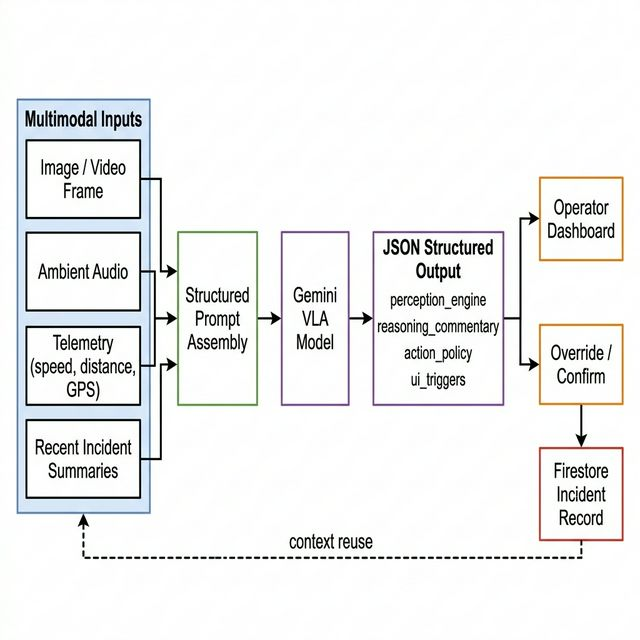
\includegraphics[width=\linewidth]{figures/system_architecture.png}
\caption{Architecture of the proposed advisory pipeline. Multimodal inputs (image, audio, telemetry, incident history) are assembled into a structured prompt, processed by the Gemini multimodal model, and produce a JSON-structured assessment consumed by the operator dashboard. Override decisions are persisted in Firestore and reused as contextual memory.}
\label{fig:architecture}
\end{figure}

\begin{figure}[t]
\centering
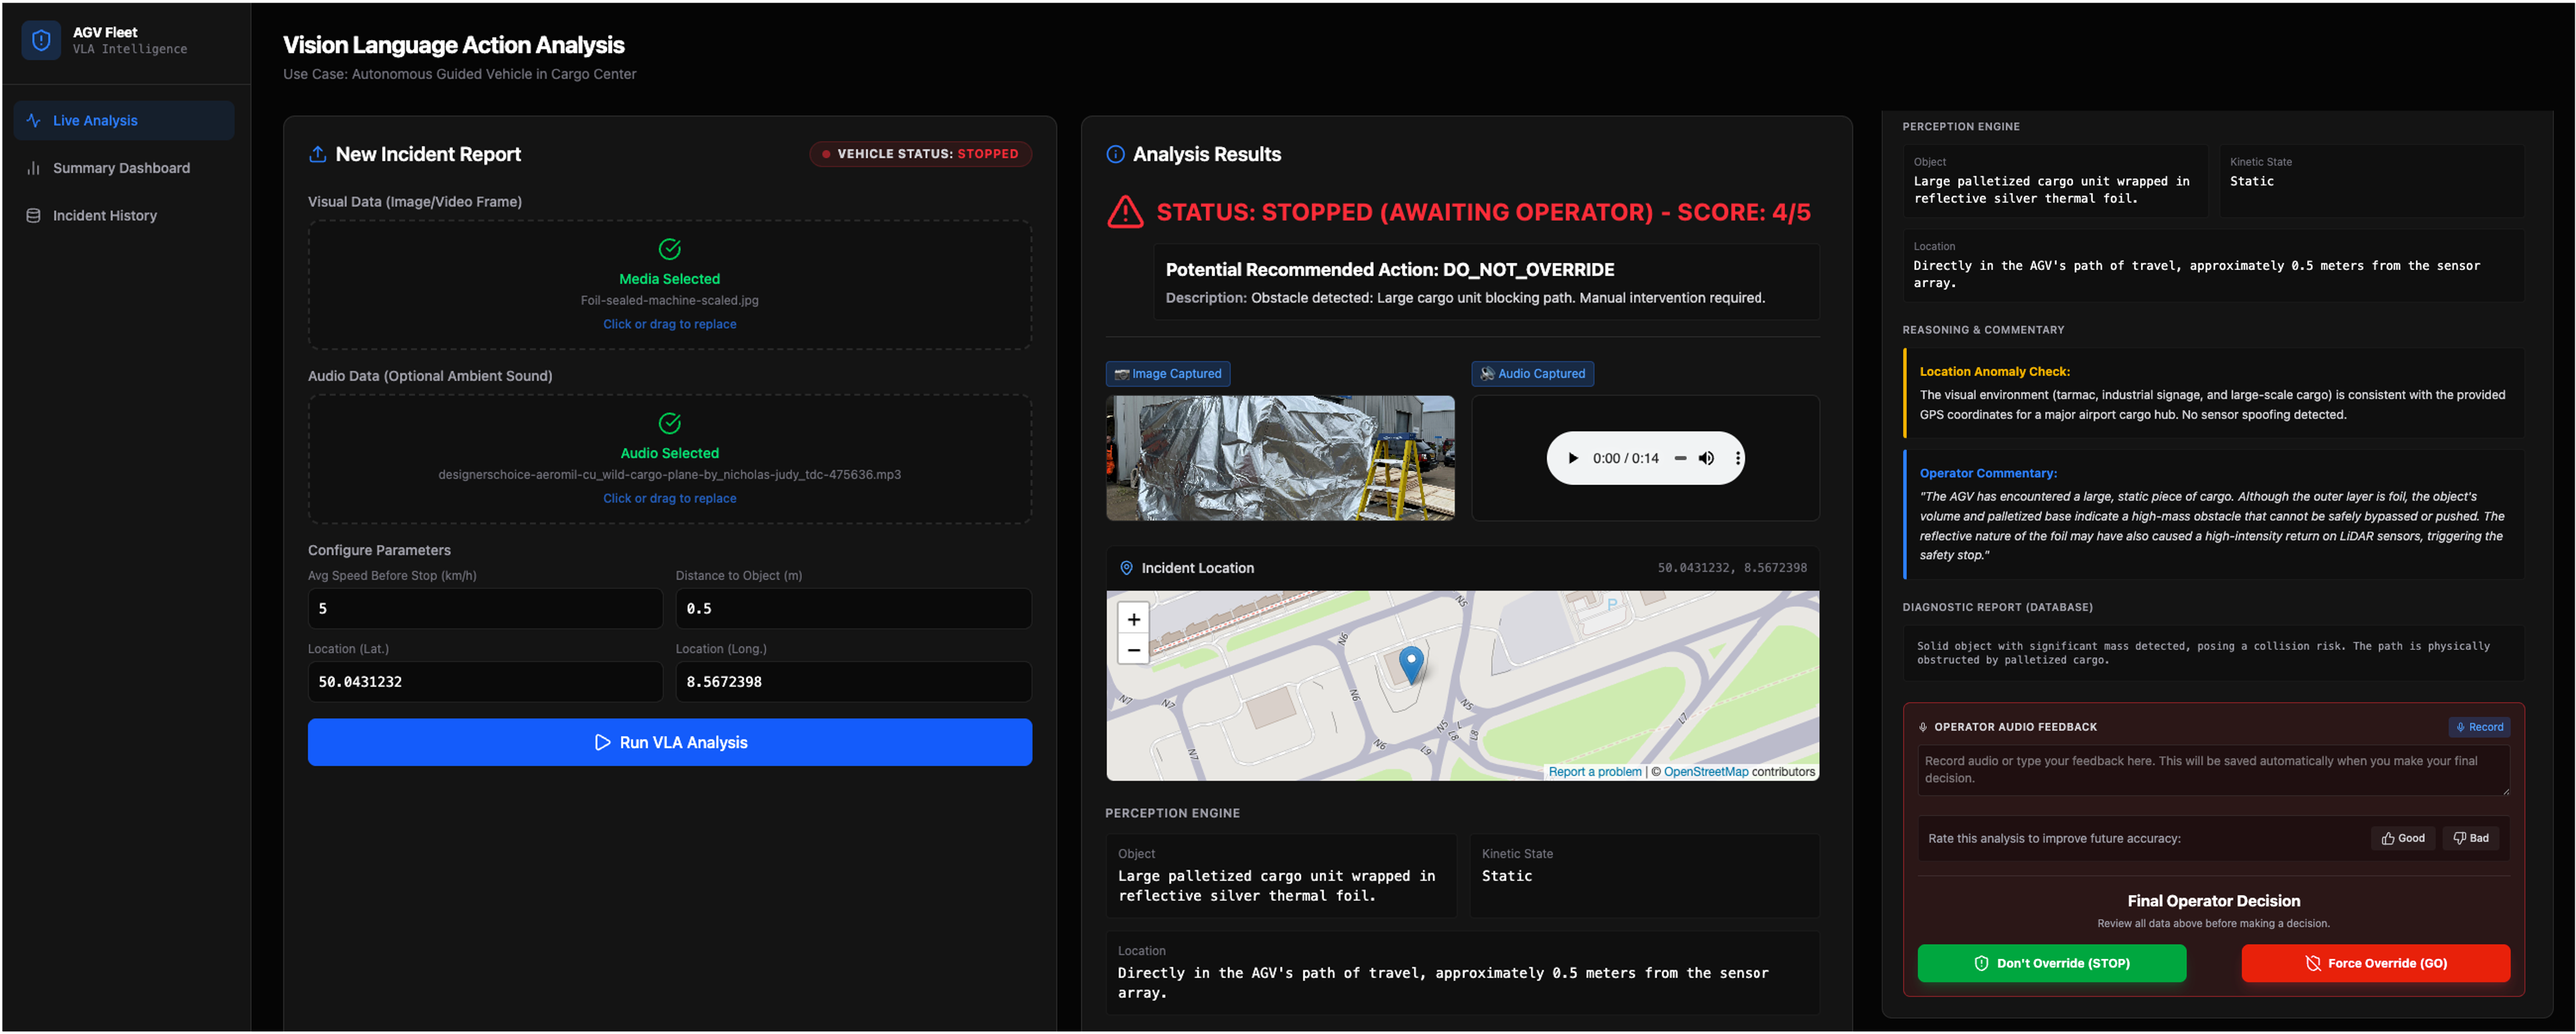
\includegraphics[width=\linewidth]{figures/dashboard_screenshot.png}
\caption{Dashboard view for live incident analysis. The interface provides visual and audio upload zones, configurable telemetry parameters (speed, distance, GPS coordinates), and a dedicated analysis results panel. The vehicle status indicator and ``Run VLA Analysis'' button support operator-initiated advisory requests.}
\label{fig:dashboard}
\end{figure}


\section{Methodology}
We frame the evaluation as a pilot study rather than a deployment study. That keeps the claims aligned with what was actually built: a working dashboard, a prompt contract, and a small benchmark, not a validated fleet system.

\subsection{Scenario Benchmark}
The long-term benchmark is intended to cover lightweight benign debris, soft hanging or drifting material, ambiguous medium-risk obstacles, solid stationary obstacles, humans or moving vehicles, and cross-modal or location-anomaly cases. The current pilot instantiates only four cases drawn from that taxonomy: a piece of aluminum foil, a plastic curtain, a wooden crate blocking the path, and an indoor-outdoor location mismatch scenario. For each case, we specify a visual scene description, optional audio cues, telemetry text, a gold danger-score range on the 1--5 scale, a binary override label, and a short rationale written before model evaluation.

Repeated or near-repeated scenarios are part of the full evaluation plan so that consistency under recent-history prompting can be measured. In the present pilot, history behavior is only spot-checked, so any conclusions about memory-assisted consistency should be treated as provisional.

\subsection{Labeling Rubric}
The benchmark uses a two-level annotation scheme. The primary label is a five-point danger score aligned with the prototype interface:
\begin{itemize}
    \item score 1: negligible risk; clearly safe to override;
    \item score 2: low risk; generally safe to override;
    \item score 3: moderate uncertainty; caution required;
    \item score 4: high risk; override discouraged;
    \item score 5: extreme risk; override prohibited.
\end{itemize}
For binary evaluation, scores 1 and 2 map to \emph{safe to override}, while scores 3, 4, and 5 map to \emph{do not override}. This mapping is intentionally conservative because ambiguous moderate-risk cases should not be counted as benign success cases in a safety-oriented study.

\subsection{Metrics and Ablations}
For a fully rerunnable benchmark, the intended quantitative metrics are binary accuracy, unsafe-case F1, danger-score mean absolute error (MAE), and repeated-scenario consistency (defined as the percentage of identical decisions when testing identical scenarios with different historical contexts). With only N=4 pilot cases, these values would still be descriptive only; one changed decision would move binary accuracy by 25 percentage points, so confidence intervals would not be meaningful at this stage.

Four ablation settings are compared in the pilot:
\begin{enumerate}
    \item vision only;
    \item vision plus telemetry;
    \item vision plus telemetry plus audio;
    \item full system with recent-history context.
\end{enumerate}
All conditions in the benchmark harness use the same system instruction, reduced structured-output contract, and deterministic decoding setting of \codefont{temperature=0.0}. In the separate text-based benchmark harness included with the prototype, the configured evaluation model is \codefont{gemini-2.5-flash}, and the response is again constrained to \codefont{application/json}. The only intended difference between ablation conditions is which modalities and contextual summaries are provided.

\begin{table}[t]
\caption{Scenario taxonomy and gold-label rubric for the full benchmark. The current pilot covers only a subset of these groups.}
\label{tab:taxonomy}
\centering
\footnotesize
\begin{tabularx}{\linewidth}{@{}lXc@{}}
\toprule
Group & Representative examples & Gold score range \\
\midrule
Benign debris & Foil, paper scraps, loose wrapping fragments, shadows & 1--2 \\
Soft material & Empty plastic bags, curtains, drifting sheets & 2--3 \\
Ambiguous objects & Unknown medium-sized objects, loose straps, cables & 3 \\
Solid obstacles & Dropped cargo, pallets, walls, parked equipment & 4 \\
Dynamic hazards & Humans, forklifts, moving vehicles, active machinery & 5 \\
Cross-modal anomalies & Audio-visual conflict, map mismatch, spoof-like cues & 3--5 \\
\bottomrule
\end{tabularx}
\end{table}

\section{Experimental Design}
The benchmark harness is structured to isolate the value of telemetry, audio, and recent-history context. The same four pilot cases can be evaluated under all four ablations described above. For each run, the analysis output is parsed into a reduced JSON structure aligned with the evaluation rubric rather than the full four-block dashboard contract. The benchmark therefore checks model judgment and reduced-schema compliance, not full end-to-end production-schema compliance.

For practicality, the pilot benchmark uses written scene descriptions and paired audio summaries rather than raw uploaded media. That is sufficient for exercising the prompt format and scoring rubric, but it is weaker than a true multimodal evaluation and should be read that way. The full dashboard can inject short summaries of up to fifteen prior incidents from Firestore. In the pilot, history context is sparse and scenario-specific, so any apparent consistency gain is suggestive rather than conclusive.

The pilot is also not directly comparable to public road-driving benchmarks such as nuScenes, Waymo, BDD100K, DriveLM, Reason2Drive, or LaMPilot-Bench \cite{caesar2020nuscenes,sun2020waymo,yu2020bdd100k,sima2024drivelm,nie2024reason2drive,ma2024lampilot}. Those resources evaluate large-scale perception, planning, or language-grounded driving on open-road data or simulation. Our evaluation instead isolates a narrow warehouse decision point: whether multimodal evidence helps an operator-facing system distinguish nuisance stops from genuine hazards.

A stronger follow-up study should also report representative examples of cross-modal stress cases. For instance, an image may appear benign while the audio suggests nearby heavy machinery, or the visual context may imply an indoor warehouse while the location string suggests a mismatched operating zone. These cases are useful because they expose precisely the kinds of failure modes that a purely vision-only analysis may miss.


\begin{figure}[t]
\centering
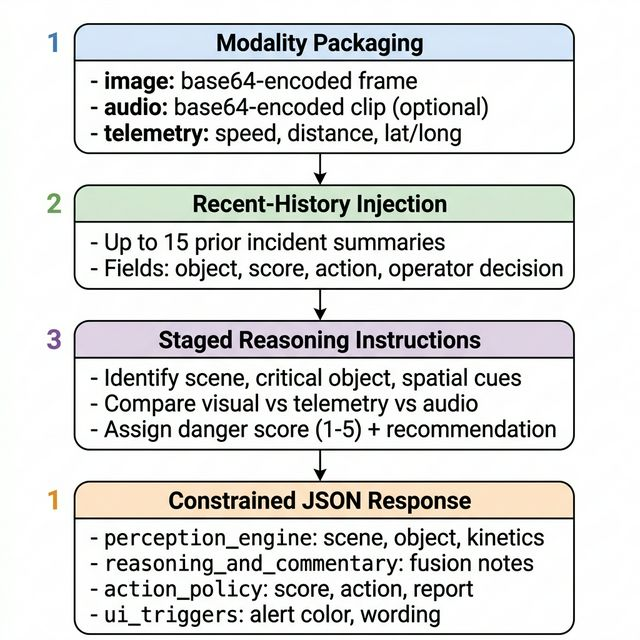
\includegraphics[width=0.85\linewidth]{figures/prompt_pipeline.png}
\caption{Prompt-to-output pipeline. Modality packaging, recent-history injection, staged reasoning instructions, and the constrained four-block JSON response consumed by the dashboard.}
\label{fig:pipeline}
\end{figure}

\section{Results and Analysis}
This section reports an offline audit of the current four-case pilot benchmark. Because the archived pilot artifacts do not currently support a reproducible model-side comparison, the focus here is on what can be verified locally and reproducibly from the scenario definitions, schema contracts, and ablation setup.

\subsection{Quantitative Reporting}
Table~\ref{tab:ablation} summarizes the measurable properties of the current pilot benchmark. Three constraints matter immediately. First, the dataset is tiny and weakly balanced: it contains one clearly safe case, one borderline case spanning the safety threshold, and two clearly unsafe cases. Second, the history mechanism is not meaningfully testable because only one case contains any historical context and there are no repeated scenario pairs. Third, the benchmark harness uses text surrogates and a reduced two-block schema, so it does not fully exercise the four-block dashboard contract used in the application.

These audit results are not a substitute for model evaluation, but they are preferable to carrying forward provisional accuracy and consistency figures that cannot currently be rerun. The table therefore functions as a claim-boundary check: it shows what the present pilot supports and what it does not.

\begin{table*}[t]
\caption{Offline audit of the current 4-case pilot benchmark. All values are computed locally from the scenario definitions and schema contracts.}
\label{tab:ablation}
\centering
\footnotesize
\begin{tabularx}{\textwidth}{@{}lcl@{}}
\toprule
Audit item & Measured value & Implication \\
\midrule
Pilot scenarios & 4 & Results are illustrative only \\
Clearly safe / borderline / clearly unsafe gold cases & 1 / 1 / 2 & Binary behavior is weakly constrained \\
Cases with non-empty history context & 1 / 4 & History effects are not generalizable \\
Explicit repeated scenario pairs & 0 & Consistency cannot be measured credibly \\
Cases using raw uploaded media in the benchmark & 0 / 4 & Pilot is text-surrogate, not full multimodal \\
Benchmark schema blocks / dashboard schema blocks & 2 / 4 & Harness under-tests the production contract \\
\bottomrule
\end{tabularx}
\end{table*}

\noindent The audit shows that the present pilot is mainly useful for checking scenario framing and interface-contract flow. It is not yet strong enough to support stable claims about modality gains, history-conditioned consistency, or failure frequency.

\subsection{Qualitative Failure Analysis}
Qualitative review still matters, but under the current constraints the more honest question is which failure modes the pilot can actually test. Unsupported anomaly claims are at least partially assessable because the benchmark includes one explicit location-mismatch case. By contrast, history bias is not meaningfully testable, and false-safe or false-danger behavior can only be weakly stressed because the pilot has just one clearly safe example.

Table~\ref{tab:failure} therefore reports failure-mode testability rather than claimed absence of failures. This reframing is more credible than asserting ``no occurrences'' when the current pilot does not contain enough repeated, history-rich, or raw-media cases to make those statements robust.

\begin{table}[t]
\caption{Failure-mode testability under the current offline pilot audit.}
\label{tab:failure}
\centering
\footnotesize
\begin{tabularx}{\linewidth}{@{}lXX@{}}
\toprule
Failure mode & Testable now? & Audit basis \\
\midrule
False-safe advisory & Limited & One clearly safe case \\
False-danger advisory & Limited & One clearly safe case and one borderline case \\
Unsupported anomaly claim & Yes & One explicit location-mismatch case \\
History bias & No & One history-enabled case and zero repeated pairs \\
Cross-modal conflict & Limited & One text-only audio/location mismatch case \\
\bottomrule
\end{tabularx}
\end{table}

\noindent The main conclusion is simple: the current pilot is useful for checking schema flow and scenario framing, not for claiming stable model performance. Any future results table should come from stored per-case outputs on a larger set with repeated-history probes and raw media inputs.

\section{Discussion}
The prototype points to a narrow but plausible role for VLA-style models in industrial autonomy: assisting with stop interpretation when the obstacle is semantically unclear, not replacing the vehicle's safety controller. That boundary matters. Using the remote-operation categories of Parr et al. \cite{parr2024remote}, the dashboard is best understood as a remote-assistance or remote-management tool rather than a remote-driving system. In the current system, the model never issues motion commands to the AGV. It produces an assessment, the operator reviews it, and the dashboard records both the recommendation and the human decision.

From an operational standpoint, the main benefit is not simply classification accuracy. It is the combination of structured explanation, historical context, and post-incident traceability. A warehouse operator dealing with repeated nuisance stops needs more than a raw score. The operator needs to know what object the system thinks it sees, why the score was assigned, whether similar incidents happened recently, and how past overrides were handled.

At the same time, the current approach has clear limitations. First, the system depends on manually uploaded evidence and typed telemetry rather than live sensor ingestion. Second, recent-history injection should be understood as prompt-conditioned contextual consistency, not learning in the statistical training sense. Third, spatial reasoning errors remain a credible risk, especially in scenes where scale, motion, or object material are hard to infer from a single frame. Finally, the current prototype does not establish formal safety guarantees, field robustness, or operator trust through user studies.

These limitations are not cosmetic caveats. They are the main claim boundaries of the paper. The value of the draft is that it turns a plausible university prototype into a research artifact with a clear architecture, a reproducible evaluation plan, and an explicit next step for stronger empirical validation.

\section{Conclusion}
This paper presented a multimodal, VLA-inspired decision-support prototype for analyzing false-positive AGV safety stops in cargo-center environments. The system combines visual media, optional audio, telemetry, and recent incident summaries to produce structured advisory output for a human operator. Its contribution is not autonomous actuation but explainable, persistent, and reviewable support for semantically difficult stop-resolution decisions.

The paper also defined a scenario-based evaluation framework and executed a preliminary four-case pilot, which is best understood as a check that the analysis, logging, and reporting workflow works as intended. Future work should expand the dataset to the planned 48--60 scenarios, replace text surrogates with raw media in the benchmark, archive per-case outputs for reproducible reruns, integrate live sensor ingestion, and study how explanation quality affects operator confidence and decision time. Those steps would move the project from an academic prototype toward a more credible industrial-assistive autonomy pipeline.

\section*{Acknowledgment}
The authors thank Peter Nauth and the Autonomous Intelligent Systems teaching staff for project guidance and feedback. The prototype implementation was developed by the authors with limited AI-assisted coding support in the Antigravity IDE using Claude Opus 4.6 (thinking) for selected implementation tasks. System design choices, evaluation framing, manuscript claims, and final verification remained the responsibility of the authors. Any remaining errors, unsupported claims, or incomplete evaluation details are the responsibility of the authors.

\bibliographystyle{IEEEtran}
\bibliography{refs}

\end{document}
